\documentclass[standalone]{beamer}

\begin{document}
\section{凹凸單調優化}

\begin{frame}{\btitle{前言}}
  \begin{itemize}
    \item 從這個章節開始,要介紹更多的 DP 優化
    \item 這章先介紹常見的 1D / 1D 優化
    \item 所謂的 $xD/yD$ 的 DP,代表說狀態是 $O(n^x)$,轉移是 $O(n^y)$ 的 DP
  \end{itemize}
\end{frame}

\begin{frame}{\btitle{問題定義}}
  \begin{theorem}[1D/1D 常見形式]
  要求的是一個一維代價 $dp[j], \;\forall\; 1\leq j\leq n$。
  給一可在常數時間內求得的轉移代價函數 (transition cost function) $f(i,j,dp[i]), \;\forall\; 0\leq i<j\leq n$、
  %可在常數時間內求得的代價 $f(i,E[i])$、
  以及初始化邊界 $dp[0]$,求:
  %\[ E[j] = \min_{0\leq i<j}\left\{f(i,E[i])+w(i,j)\right\}, \;\forall\; 1\leq i\leq n \]
  \[ dp[j] = \min_{0\leq i<j}\left\{f(i,j,dp[i])\right\}, \;\forall\; 1\leq j \leq n \]
  \end{theorem}
  接下來為了討論方便,我們把 $f(i,j,dp[i])$ 簡單寫作 $f(i,j)$

  不過討論時須注意 $f(i,j)$ 事實上和 $dp[i]$ 有關,因此他是\textbf{在線 (online)} 的,也就是 $f(i,j)$的值必須在 $dp[i]$ 被計算出來後才能得知
\end{frame}

\begin{frame}{\btitle{單調性}}
  \begin{figure}[h]
  \begin{minipage}[c]{0.33\linewidth}
  \begin{center}
  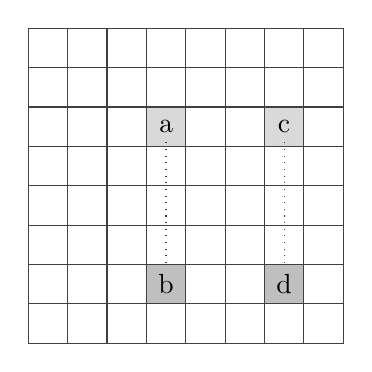
\begin{tikzpicture}
    %\draw[draw=black!75, fill=white] (\x,\y) rectangle ++(0.5,0.5); 
    \fill[color=black!15] (1.5,2.5) +(-.25,-.25) rectangle ++(.25,.25); 
    \draw (1.5,2.5) node (a) {a};
    \fill[color=black!15] (3.0,2.5) +(-.25,-.25) rectangle ++(.25,.25); 
    \draw (3.0,2.5) node (c) {c};
    \fill[color=black!25] (1.5,0.5) +(-.25,-.25) rectangle ++(.25,.25); 
    \draw (1.5,0.5) node (b) {b};
    \fill[color=black!25] (3.0,0.5) +(-.25,-.25) rectangle ++(.25,.25); 
    \draw (3.0,0.5) node (d) {d};
    
    \foreach \y in {0,0.5,...,3.5} {
        \foreach \x in {0,0.5,...,3.5} {
          \draw[draw=black!75, fill=white, fill opacity=0.0] (\x,\y) +(-.25,-.25) rectangle ++(.25,.25); 
        }
    }
    \draw[draw=black!75,dotted] (a) -- (b);
    \draw[draw=black!75,dotted] (c) -- (d);
  \end{tikzpicture}
  \end{center}
  \end{minipage}
  \begin{minipage}[c]{0.67\linewidth}
  % $\forall \;a=A[i_1][j_1], b=A[i_2][j_1], c=A[i_1][j_2], d=A[i_2][j_2]$,\\
  % 其中 $i_1<i_2, j_1<j_2$:

  % FIXME: temporary paragraph spacing hack, fix if possible
  \setlength{\abovedisplayskip}{0pt}
  \setlength{\belowdisplayskip}{0pt}
  凹單調(concave totally monotone):
  $$a\leq b \Rightarrow c\leq d$$

  凸單調(convex totally monotone):
  $$a\geq b \Rightarrow c\geq d$$
  \end{minipage}
  \end{figure}

\end{frame}

\begin{frame}{\btitle{單調性}}
  \begin{itemize}
    \item 假設 $i_1 < i_2, j_1 < j_2$:
    \item 凹單調:若 $A[i_1][j_1] \leq A[i_2][j_1]$ 則 $A[i_1][j_2] \leq A[i_2][j_2]$
    \item 凸單調:若 $A[i_1][j_1] \geq A[i_2][j_1]$ 則 $A[i_1][j_2] \geq A[i_2][j_2]$
    \item 代表最佳選擇具有某種程度的「淘汰性」,也就是某個時間點後一個選擇一旦輸給了某個順序在他之前/後的選擇,他就再也不可能是最佳的選擇
  \end{itemize}
\end{frame}


\begin{frame}{\btitle{凹單調}}
  \begin{figure}[h]
  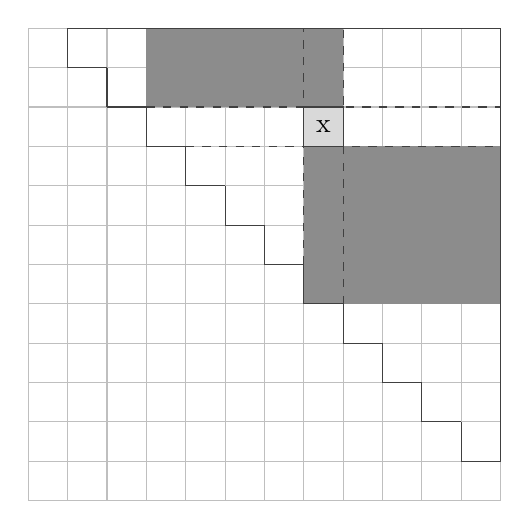
\begin{tikzpicture}
    \foreach \y in {0,0.5,...,5.5} {
        \foreach \x in {0,0.5,...,5.5} {
        \pgfmathsetmacro{\sumxy}{\x+\y};
            \ifthenelse{\lengthtest{\sumxy pt<5.6pt}}{
              \draw[draw=black!10, fill=white] (\x,\y) rectangle ++(0.5,0.5); 
            } {
                \draw[draw=black!25, fill=white] (\x,\y) rectangle ++(0.5,0.5); 
            }
        }
    }
    %
    \foreach \x in {3.5,4.0,...,5.5} {
        \foreach \y in {2.5,3.0,...,4.0} {
        \pgfmathsetmacro{\sumxy}{\x+\y};
            \ifthenelse{\lengthtest{\sumxy pt<5.6pt}}{
            } {
                \draw[draw opacity=0, fill=black!45] (\x,\y) rectangle ++(0.5,0.5); 
            }
        }
    }
    \foreach \x in {1.5,2.0,...,3.5} {
        \foreach \y in {5.0,5.5} {
        \pgfmathsetmacro{\sumxy}{\x+\y};
            \ifthenelse{\lengthtest{\sumxy pt<5.6pt}}{
            } {
                \draw[draw opacity=0, fill=black!45] (\x,\y) rectangle ++(0.5,0.5); 
            }
        }
    }
    %
    \draw[draw=black!75] (0.5,6) -- (6,6);
    \draw[draw=black!75] (6,0.5) -- (6,6);
    \foreach \x in {0.5,1.0,...,5.5} {
      \draw[draw=black!75] (\x,6.5-\x) -- (\x,6.0-\x);
      \draw[draw=black!75] (\x,6.0-\x) -- (\x+0.5,6.0-\x);
    }
    \draw[draw=black!75,dashed] (3.5,3.0) -- (3.5,6.0);
    \draw[draw=black!75,dashed] (4.0,2.5) -- (4.0,6.0);
    \draw[draw=black!75,dashed] (1.5,5.0) -- (6.0,5.0);
    \draw[draw=black!75,dashed] (2.0,4.5) -- (6.0,4.5);
    \draw[draw=black!75,fill=black!15] (3.5,4.5) rectangle ++(0.5,0.5);
    \draw (3.75,4.75) node (x) {x};
  \end{tikzpicture}
  \caption{凹單調時,被 x 殺死的元素}
  \end{figure}
\end{frame}

\begin{frame}{\btitle{凹單調}}
  \begin{figure}[h]
  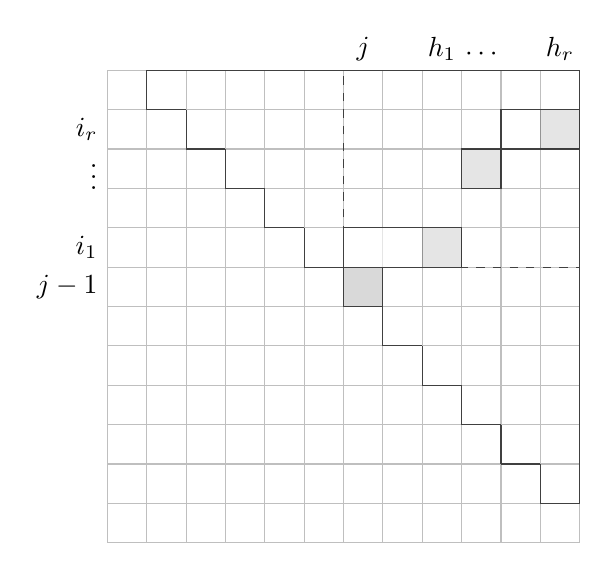
\begin{tikzpicture}
    \foreach \y in {0,0.5,...,5.5} {
        \foreach \x in {0,0.5,...,5.5} {
        \pgfmathsetmacro{\sumxy}{\x+\y};
          %\ifthenelse{\lengthtest{\sumxy pt<5.4pt}}{\def\mycol{black!15}}{\def\mycol{white}}
            %\draw[draw=black!75, fill=\mycol] (\x,\y) rectangle ++(0.5,0.5); 
            \ifthenelse{\lengthtest{\sumxy pt<5.6pt}}{
              \draw[draw=black!10, fill=white] (\x,\y) rectangle ++(0.5,0.5); 
            } {
                \draw[draw=black!25, fill=white] (\x,\y) rectangle ++(0.5,0.5); 
            }
        }
    }
    \draw[draw=black!75] (0.5,6) -- (6,6);
    \draw[draw=black!75] (6,0.5) -- (6,6);
    \foreach \x in {0.5,1.0,...,5.5} {
      \draw[draw=black!75] (\x,6.5-\x) -- (\x,6.0-\x);
      \draw[draw=black!75] (\x,6.0-\x) -- (\x+0.5,6.0-\x);
    }
    \draw[draw=black!75,dashed] (3.0,3.5) -- (3.0,6.0);
    \draw[draw=black!75,dashed] (3.0,3.5) -- (6.0,3.5);
    \draw[draw=black!75,fill=black!15] (3.0,3.0) rectangle (3.5,3.5);
    \draw[draw=black!75,fill=white,fill opacity=0.6] (3.0,3.5) rectangle (4.5,4.0);
    \draw[draw=black!75,fill=black,draw opacity=0.4,fill opacity=0.1] (4.0,3.5) rectangle (4.5,4.0);
    \draw[draw=black!75,fill=white,fill opacity=0.6] (4.5,4.5) rectangle (5.0,5.0);
    \draw[draw=black!75,fill=black,draw opacity=0.4,fill opacity=0.1] (4.5,4.5) rectangle (5.0,5.0);
    \draw[draw=black!75,fill=white,fill opacity=0.6] (5.0,5.0) rectangle (6.0,5.5);
    \draw[draw=black!75,fill=black,draw opacity=0.4,fill opacity=0.1] (5.5,5.0) rectangle (6.0,5.5);
    %
    \node [anchor=east] at (0,3.25) {$j-1$};
    \node [anchor=east] at (0,3.75) {$i_1$};
    \node [anchor=east] at (0,4.75) {$\vdots$};
    \node [anchor=east] at (0,5.25) {$i_r$};
    %
    \node [anchor=south] at (3.25,6) {$j$};
    \node [anchor=south] at (4.25,6) {$h_1$};
    \node [anchor=south] at (4.75,6) {$\cdots$};
    \node [anchor=south] at (5.75,6) {$h_r$};
  \end{tikzpicture}
  \caption{凹單調性 DP}
  \end{figure}
\end{frame}

\begin{frame}{\btitle{凹單調}}
  \begin{itemize}
    \item 用\textbf{列區間(row segment)}來代表這些人選
    \item $S = ([i_1,j:h_1],[i_2,h_1+1:h_2],\dots,[i_k,h_{k-1}+1:h_k])$
    \item 其中 $[i,j_1:j_2]$ 代表第 $i$ 列上,第 $j_1$ 到第 $j_2$ 行所形成的列區間,$h_t$ 是第 $t$ 個列區間的最右元素
  \end{itemize}
\end{frame}

\begin{frame}[fragile]{\btitle{凹單調}}
  \begin{minted}[breaklines]{cpp}
    stack<Seg> sta;
    sta.push(Seg(0, 1, m));
    for (int j = 1; j <= m; ++j) {
      while (!sta.empty() && sta.top().r < j) sta.pop(); // 把過期的最佳解丟掉
      dp[j] = cal(sta.top().pos, j);
      
      while (!sta.empty() && cal(sta.top().pos, sta.top().r) > cal(j, sta.top().r)) {
        // 把被完全覆蓋的線段刪掉
        sta.pop();
      }
      if (sta.empty()) {
        sta.push(Seg(j, j + 1, m));
      }
  \end{minted}
\end{frame}

\begin{frame}[fragile]{\btitle{凹單調}}
  \begin{minted}[breaklines]{cpp}
      else {
        Seg seg = sta.top(); sta.pop();
        // 二分搜斷點
        int l = seg.l - 1, r = seg.r;
        while (r - l > 1) {
          int mid = (l + r) >> 1;
          if (cal(seg.pos, mid) >= cal(j, mid)) l = mid;
          else r = mid;
        }
        sta.push(Seg(seg.pos, r, seg.r));
        if (j + 1 <= l) sta.push(Seg(j, j + 1, l));
      }
    }
  \end{minted}
\end{frame}



\begin{frame}{\btitle{凸單調}}
  \begin{figure}[h]
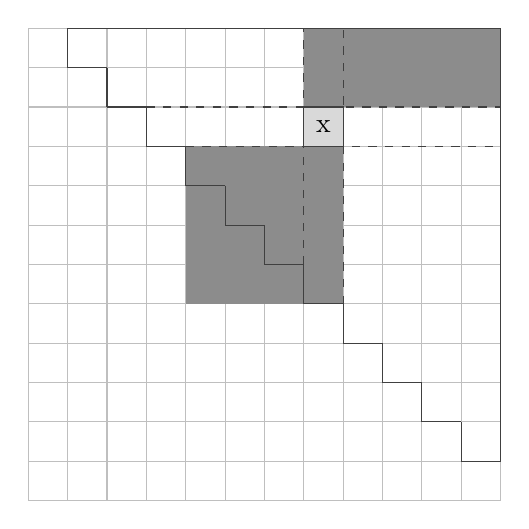
\begin{tikzpicture}
  \foreach \y in {0,0.5,...,5.5} {
      \foreach \x in {0,0.5,...,5.5} {
      \pgfmathsetmacro{\sumxy}{\x+\y};
          \ifthenelse{\lengthtest{\sumxy pt<5.6pt}}{
            \draw[draw=black!10, fill=white] (\x,\y) rectangle ++(0.5,0.5); 
          } {
              \draw[draw=black!25, fill=white] (\x,\y) rectangle ++(0.5,0.5); 
          }
      }
  }
  %
  \foreach \x in {2.0,2.5,...,3.5} {
      \foreach \y in {2.5,3.0,...,4.0} {
      \pgfmathsetmacro{\sumxy}{\x+\y};
          \ifthenelse{\lengthtest{\sumxy pt<5.6pt}}{
          } {
              \draw[draw opacity=0, fill=black!45] (\x,\y) rectangle ++(0.5,0.5); 
          }
      }
  }
  \foreach \x in {3.5,4,...,5.5} {
      \foreach \y in {5.0,5.5} {
          \draw[draw opacity=0, fill=black!45] (\x,\y) rectangle ++(0.5,0.5); 
      }
  }
  %
  \draw[draw=black!75] (0.5,6) -- (6,6);
  \draw[draw=black!75] (6,0.5) -- (6,6);
  \foreach \x in {0.5,1.0,...,5.5} {
    \draw[draw=black!75] (\x,6.5-\x) -- (\x,6.0-\x);
    \draw[draw=black!75] (\x,6.0-\x) -- (\x+0.5,6.0-\x);
  }
  \draw[draw=black!75,dashed] (3.5,3.0) -- (3.5,6.0);
  \draw[draw=black!75,dashed] (4.0,2.5) -- (4.0,6.0);
  \draw[draw=black!75,dashed] (1.5,5.0) -- (6.0,5.0);
  \draw[draw=black!75,dashed] (2.0,4.5) -- (6.0,4.5);
  \draw[draw=black!75,fill=black!15] (3.5,4.5) rectangle ++(0.5,0.5);
  \draw (3.75,4.75) node (x) {x};
\end{tikzpicture}  \caption{凸單調時,被 x 殺死的元素}
  \end{figure}
\end{frame}

\begin{frame}{\btitle{凸單調}}
  \begin{figure}[h]
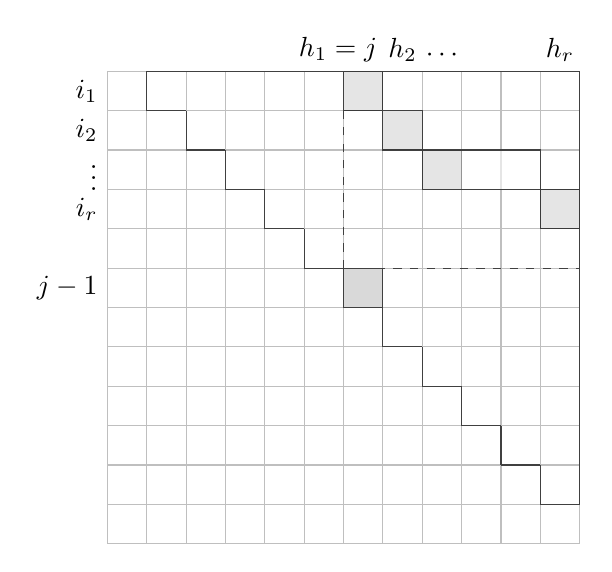
\begin{tikzpicture}
  \foreach \y in {0,0.5,...,5.5} {
      \foreach \x in {0,0.5,...,5.5} {
      \pgfmathsetmacro{\sumxy}{\x+\y};
        %\ifthenelse{\lengthtest{\sumxy pt<5.4pt}}{\def\mycol{black!15}}{\def\mycol{white}}
          %\draw[draw=black!75, fill=\mycol] (\x,\y) rectangle ++(0.5,0.5); 
          \ifthenelse{\lengthtest{\sumxy pt<5.6pt}}{
            \draw[draw=black!10, fill=white] (\x,\y) rectangle ++(0.5,0.5); 
          } {
              \draw[draw=black!25, fill=white] (\x,\y) rectangle ++(0.5,0.5); 
          }
      }
  }
  \draw[draw=black!75] (0.5,6) -- (6,6);
  \draw[draw=black!75] (6,0.5) -- (6,6);
  \foreach \x in {0.5,1.0,...,5.5} {
    \draw[draw=black!75] (\x,6.5-\x) -- (\x,6.0-\x);
    \draw[draw=black!75] (\x,6.0-\x) -- (\x+0.5,6.0-\x);
  }
  \draw[draw=black!75,dashed] (3.0,3.5) -- (3.0,6.0);
  \draw[draw=black!75,dashed] (3.0,3.5) -- (6.0,3.5);
  \draw[draw=black!75,fill=black!15] (3.0,3.0) rectangle (3.5,3.5);
  \draw[draw=black!75,fill=white,fill opacity=0.6] (3.0,5.5) rectangle (3.5,6.0);
  \draw[draw=black!75,fill=black,draw opacity=0.4,fill opacity=0.1] (3.0,5.5) rectangle (3.5,6.0);
  \draw[draw=black!75,fill=white,fill opacity=0.6] (3.5,5.0) rectangle (4.0,5.5);
  \draw[draw=black!75,fill=black,draw opacity=0.4,fill opacity=0.1] (3.5,5.0) rectangle (4.0,5.5);
  \draw[draw=black!75,fill=white,fill opacity=0.6] (4.0,4.5) rectangle (5.5,5.0);
  \draw[draw=black!75,fill=black,draw opacity=0.4,fill opacity=0.1] (4.0,4.5) rectangle (4.5,5.0);
  \draw[draw=black!75,fill=white,fill opacity=0.6] (5.5,4.0) rectangle (6.0,4.5);
  \draw[draw=black!75,fill=black,draw opacity=0.4,fill opacity=0.1] (5.5,4.0) rectangle (6.0,4.5);
  %
  \node [anchor=east] at (0,3.25) {$j-1$};
  \node [anchor=east] at (0,5.75) {$i_1$};
  \node [anchor=east] at (0,5.25) {$i_2$};
  \node [anchor=east] at (0,4.75) {$\vdots$};
  \node [anchor=east] at (0,4.25) {$i_r$};
  %
  \node [anchor=south east] at (3.55,6) {$h_1=j$};
  \node [anchor=south] at (3.75,6) {$h_2$};
  \node [anchor=south] at (4.25,6) {$\cdots$};
  \node [anchor=south] at (5.75,6) {$h_r$};
\end{tikzpicture}
  \caption{凸單調性 DP}
  \end{figure}
\end{frame}

\begin{frame}{\btitle{凸單調}}
  \begin{itemize}
    \item 用\textbf{列區間(row segment)}來代表這些人選
    \item $S = ([i_1,j:h_1],[i_2,h_1+1:h_2],\dots,[i_k,h_{k-1}+1:h_k])$
    \item 其中 $[i,j_1:j_2]$ 代表第 $i$ 列上,第 $j_1$ 到第 $j_2$ 行所形成的列區間,$h_t$ 是第 $t$ 個列區間的最右元素
  \end{itemize}
\end{frame}

\begin{frame}[fragile]{\btitle{凸單調}}
  \begin{minted}[breaklines]{cpp}
    deque<Seg> dq;
    dq.push_back(Seg(0, 1, n));
    for (int j = 1; j <= n; ++j) {
      while (!dq.empty() && dq[0].r < j) dq.pop_front(); // 把過期的最佳解丟掉
      dp[j] = cal(dq[0].pos, j);
      while (!dq.empty() && cal(dq.back().pos, dq.back().l) > cal(j, dq.back().l)) {
        // 把被完全覆蓋的線段刪掉
        dq.pop_back();
      }
      if (dq.empty()) {
        dq.push_back(Seg(j, j + 1, n));
      }
  \end{minted}
\end{frame}

\begin{frame}[fragile]{\btitle{凸單調}}
  \begin{minted}[breaklines]{cpp}
      else {
        Seg seg = dq.back(); dq.pop_back();
        // 二分搜斷點
        int l = seg.l, r = seg.r + 1;
        while (r - l > 1) {
          int mid = (l + r) >> 1;
          if (cal(seg.pos, mid) > cal(j, mid)) r = mid;
          else l = mid;
        }
        dq.push_back(Seg(seg.pos, seg.l, l));
        if (l != n) dq.push_back(Seg(j, l + 1, n));
      }
    }
  \end{minted}
\end{frame}

\begin{frame}{\btitle{Monge Condition}}
  \begin{theorem}[Monge condition]
    給一個$m \times n$ 矩陣 $B$,若 $\forall 1\leq i_1<i_2 \leq m, 1\leq j_1<j_2\leq n$我們有:
    $$B[i_1][j_1]+B[i_2][j_2] \;\;\leq (\geq)\;\; B[i_1][j_2]+B[i_2][j_1]$$
    那我我們說他符合 convex (concave) Monge condition.
  \end{theorem}
  \begin{theorem}[Monge condition (等價形式)]
    給一個$m \times n$ 矩陣 $B$,若 $\forall 1\leq i<m, 1\leq j< n$我們有:
    $$B[i][j]+B[i+1][j+1] \;\;\leq (\geq)\;\; B[i][j+1]+B[i+1][j]$$
    那我我們說他符合 convex (concave) Monge condition.
  \end{theorem}
\end{frame}

\begin{frame}{\btitle{Monge Condition}}
  \begin{itemize}
    \item 容易驗證,由 convex (concave) Monge condition 推得凸(凹)單調性(也就是說,凹凸單調優化的正確性常用 Monge condition 證明)
    \item 要注意的是,Monge condition 事實上是比較嚴格的,因此\textbf{反方向的推論並不成立},不符合 Monge condition 也不代表不具有單調性
  \end{itemize}
\end{frame}

\end{document}
